1. $\cfrac{(x^2+5x-14)(x-3)^2}{|x+1|}\leqslant0\Leftrightarrow\cfrac{(x+7)(x-2)(x-3)^2}{|x+1|}\leqslant0.$ Применив метод интервалов, найдём ответ:
\begin{figure}[ht!]
\center{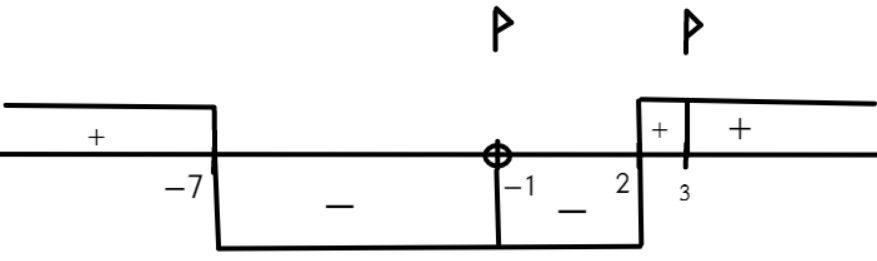
\includegraphics[scale=0.35]{int1.png}}
\end{figure}
$x\in[-7;-1)\cup(-1;2]\cup\{3\}.$\\
